\section{Mesh-Netze (ca. 1 Seite)}

Bei einem Mesh-Netz (vermaschten Netzt) handelt es sich um eine Netzwerktopologie. Das Netzwerk kann entweder aus drahtgebunden oder drahtlosen Netzwerkgeräten bestehen. In weiteren Verlauf werden nur drahtlose Netzwerkgeräte betrachtet. Bei einem Mesh-Netz können alle Netzwerkknoten genutzt werden um Daten von Punkt A zu Punkt B zu übertragen. 
\begin{figure}
	\centering
	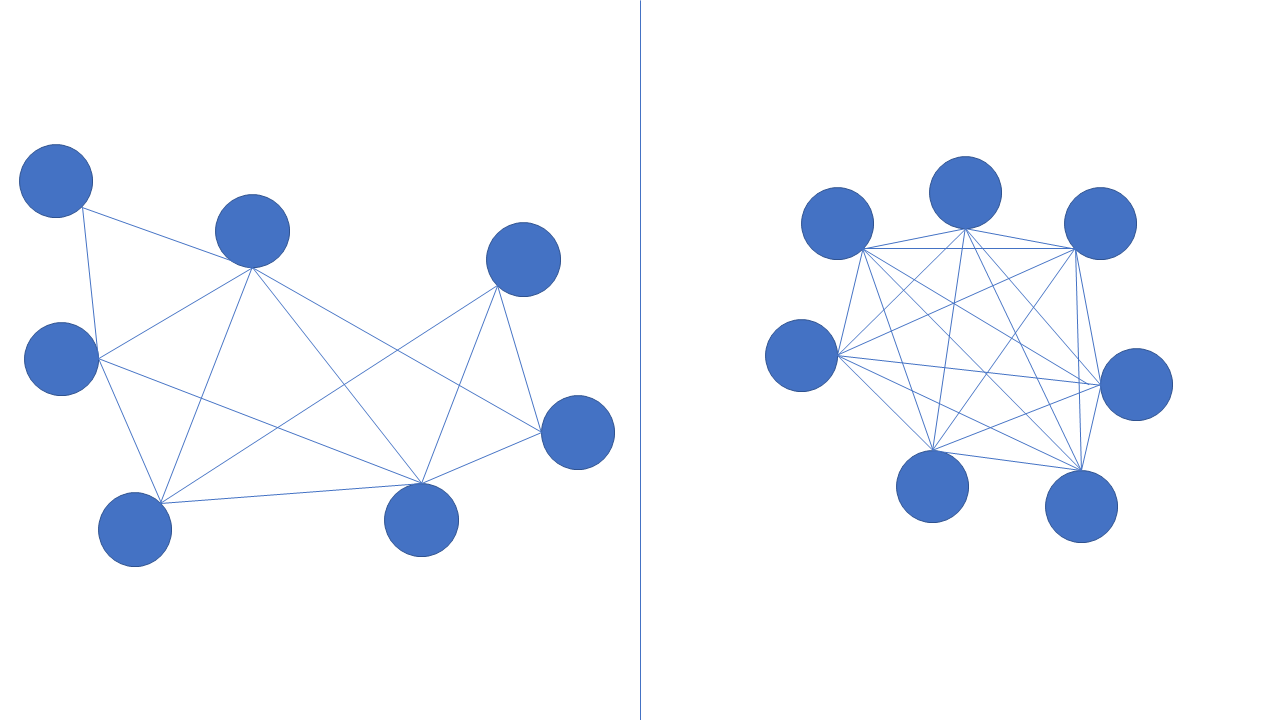
\includegraphics[width=0.9\textwidth]{bilder/vermaschtesNetz.png}
	\caption{ Mesh Netzwerk Topologie }
	\label{img:vermaschtesNetz}
\end{figure}


Von einem Mesh Netz wird gesprochen wenn jedes Netzwerkgerät mit mindestens einem oder mehreren Netzwerkgeräten verbunden ist(siehe linke Hälfte der Grafik \ref{img:vermaschtesNetz}). In der Literatur wird meist erst von einem Mesh Netz gesprochen, wenn das Netzwerkgerät über zwei unabhängige Pfade erreicht werden kann. Und wenn jedes Netzwerkgerät mit jedem Netzwerkgerät verbunden ist, wird von einem vollständig vermaschtem Netz gesprochen (siehe rechte Hälfte der Grafik \ref{img:vermaschtesNetzt}). Ein Beispiel für ein teilweise vermaschtes Netzt ist das Internet. 
Bei einem Ausfall eines Knotens/Netzwerkgerät im Mesh Netz können die Daten der anderen Netzwerkgeräte trotzdem an ihr Ziel gelangen. Deshalb ist das Netzt vor allem hinsichtlich seine Ausfallwahrscheinlichkeit deutlich erhöht, im Gegensatz zu anderen Netzwerktopologien ( zum Beispiel Stern-Topologie).  Zusätzlich benötigt ein Mesh Netz keine zentrale Verwaltung, die den Datenfluss steuert.
Ein Mesh Netz bietet die typischen Netzwerkaufgaben:
\begin{itemize}
	\item Wegsuche (Routing)
	\item Überlastkontrolle (Congestion Control)
	\item Flußkontrolle (Flow Control)
\end{itemize}

In einem Mesh Netzwerk ist das Routing einer der größten Herausforderungen \textbf{TODO}: Routing: Reactive Active Hybrid
